\section{Antecedentes}

\begin{frame}
	\frametitle{Desalinizador autónomo}
	En 2018 se desarrolló un destilador solar activo e híbrido, capaz de destilar hasta \SI{10}{\litre} por día en días soleados usando precalentamiento de agua\\
	\begin{figure}
		\centering
		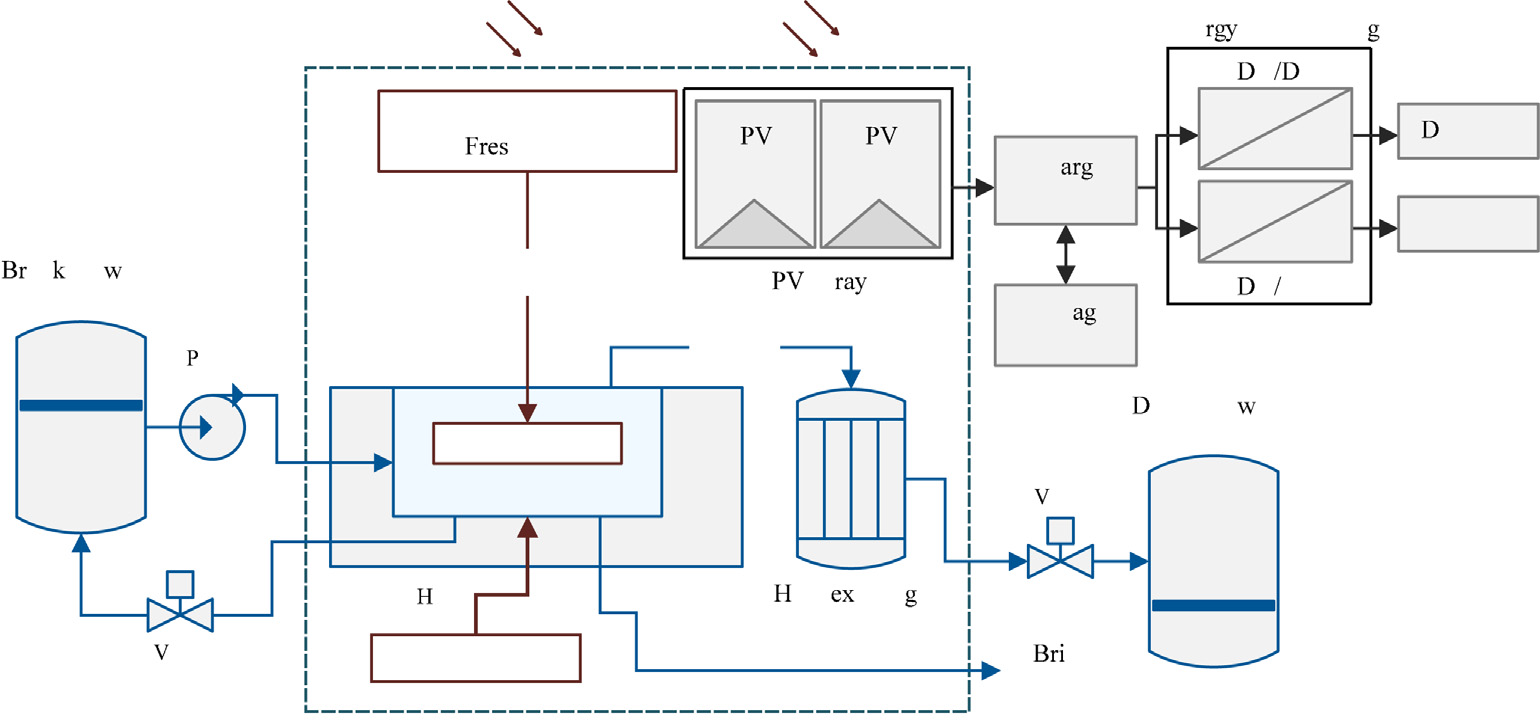
\includegraphics[
			height=45mm,
			width=\linewidth,
			keepaspectratio
		]{destilador-palomino.png}
		\caption{Destilador solar activo de Palomino et. al}
		{\scriptsize\fullcite{palomino-resendiz_design_2018}}
	\end{figure}
\end{frame}


\begin{frame}
	\frametitle{Desalinizador de doble cámara}
	En 2022 se desarrolló un destilador solar activo el cual tuvo una producción de \qty{4.03}{\litre\per\metre\tothe{2}} por día.\\
	\begin{figure}
		\centering
		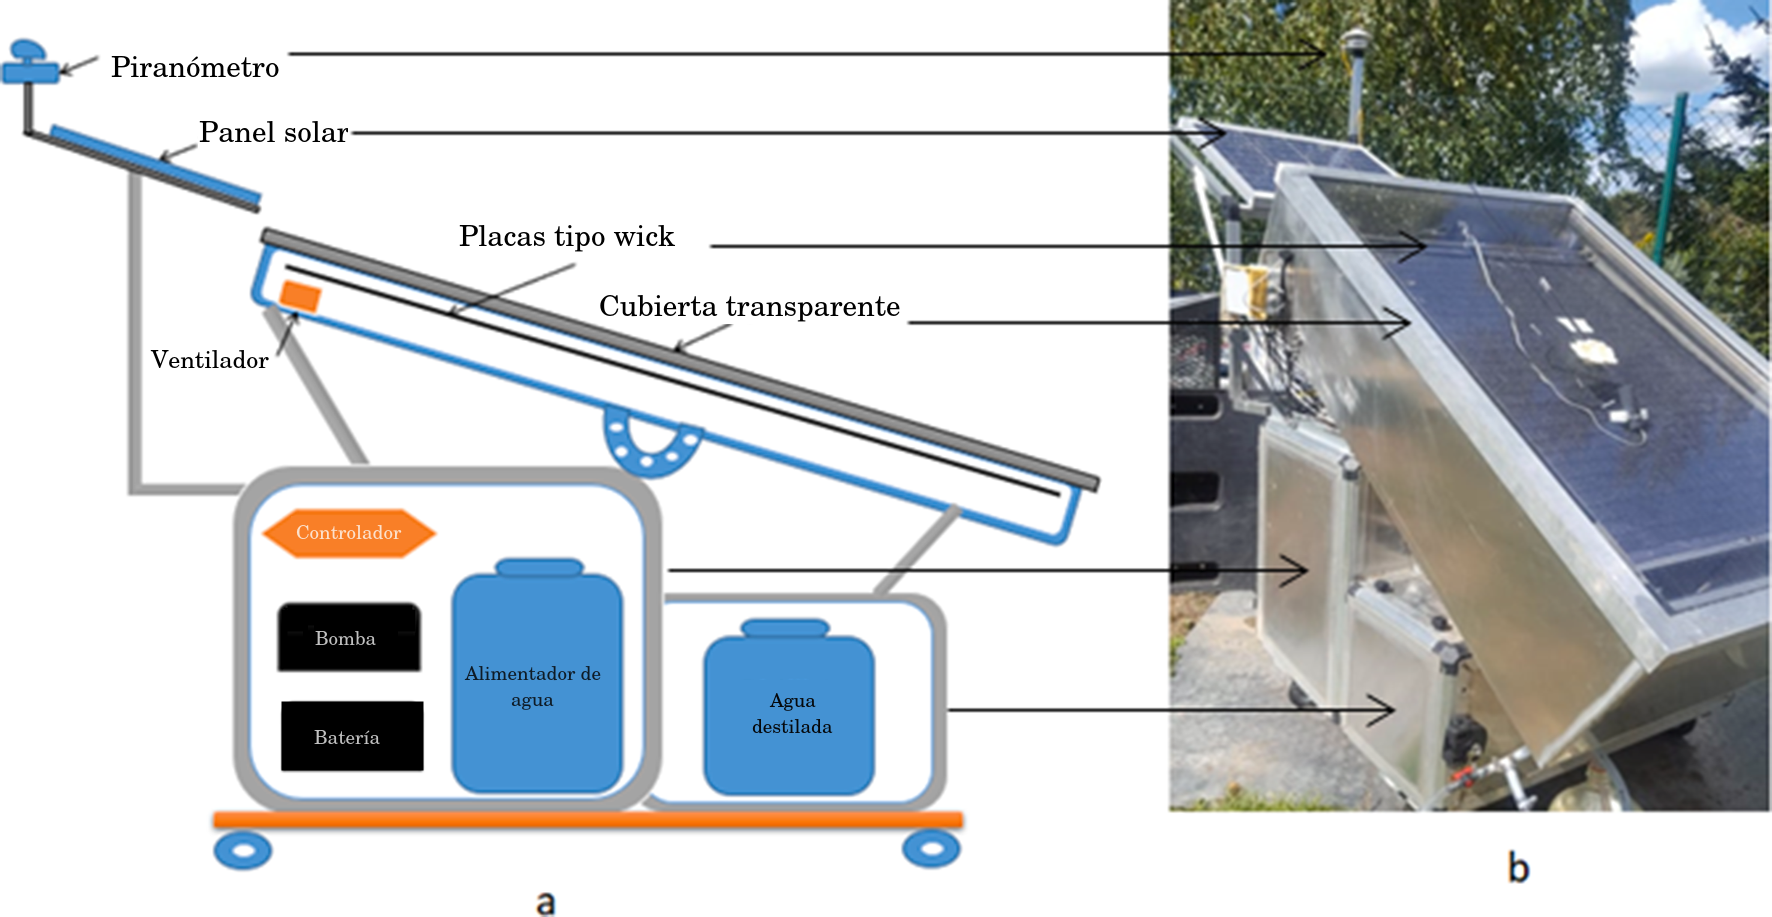
\includegraphics[
			height=45mm,
			width=\linewidth,
			keepaspectratio
		]{solar-wick-distiller.png}
		\caption{Destilador solar de doble cámara}
		{\scriptsize\fullcite{jobrane_theoretical_2022}}
	\end{figure}
\end{frame}